

\documentclass[conference]{IEEEtran}



\usepackage{comment}
\usepackage{listings}



\usepackage{url}


\usepackage{code}
\usepackage{graphicx}



% correct bad hyphenation here
\hyphenation{op-tical net-works semi-conduc-tor}


\begin{document}
\title{Falsification-Driven Verification}

\author{\IEEEauthorblockN{Alex Groce, Iftekhar Ahmed, Carlos Jensen}
\IEEEauthorblockA{School of Electrical Engineering and Computer  Science\\
Oregon State University, Corvallis, Oregon\\
Email: agroce@gmail.com, ahmedi@onid.oregonstate.edu, cjensen@eecs.orst.edu}
\and
\IEEEauthorblockN{Paul E. McKenney}
\IEEEauthorblockA{IBM Linux Technology Center\\
Email: paulmck@linux.vnet.ibm.com}
}


\maketitle


\begin{abstract}
Formal verification has finally advanced to a state where non-experts, including systems software developers, may want to verify the correctness of small but critical modules.  Unfortunately, despite considerable efforts in the area, determining if a ``verification'' actually verifies what the author intends it to is still difficult, even for model checking experts.  Previous approaches from the model checking community are valuable, but difficult to understand and limited in applicability.  Developers using a tool like a bounded model checker need verification coverage in terms of the software they are verifying, rather than in model checking terms.  In this paper we propose a tool framework and methodology to allow both developers and expert users to determine, more precisely, just what it is that they have verified for software systems.  Our basic approach is based on a novel variation of mutation analysis and a conceptual model of verification based on Popper's notion of falsification.  We use the popular C/C++ bounded model checker CBMC, modified to allow a user to determine the ``strength'' of a mutant, and show that this approach is applicable not only to simple (but complete, within bounds) verification of data structures and sorting routines, and verification of a routine in Mozilla's JavaScript engine, but to understanding an ongoing effort to verify the Linux kernel Read-Copy-Update mechanism.

\end{abstract}

\IEEEpeerreviewmaketitle



\section{Introduction}

Software model checking \cite{ModelChecking} has recently, thanks to
improvements in model checking tools as well as SAT and SMT solvers,
and the large amount of memory available even on commodity
workstations, become a potentially valuable tool for developers of
critical software modules who want to, at minimum, perform a very
aggressive search for bugs and, at best, prove correctness of their
code.  Tools such as CBMC \cite{CBMCp} (the C Bounded Model Checker)
allow a software engineer to model check code by writing what is
essentially a generalized test harness\footnote{By a harness we mean a
  program that defines an environment and the form of valid tests, and provides correctness
  properties.} in the language of the
Software Under Test (SUT).  Figure \ref{fig:sortharness} shows an
example CBMC harness for sorting routines.  Only a few aspects differ
from normal testing.  First, {\tt nondet\_int} in CBMC can return
\emph{any value}.  It is not equivalent to a ``random''
choice but true nondeterminism: CBMC will explore all values of the type.
The {\tt \_\_CPROVER\_assume} statement is used to restrict
program executions: it has the usual {\tt assume} semantics
\cite{EWD:Discipline,exploit}, so CBMC ignores all executions that
violate assumptions.

\begin{figure}
{\scriptsize
\begin{code}
\#include "sort.h"

int a[SIZE];
int ref[SIZE];

int nondet\_int();

int main () \{
  int i, v, prev;
  int s = nondet\_int();
  \_\_CPROVER\_assume((s > 0) \&\& (s <=SIZE));
  for (i = 0; i < s; i++) \{
    v = nondet\_int();
    printf ("LOG: ref[\%d] = \%d\\n", i, v);
    ref[i] = v; a[i] = v;
  \}
  sort(a, s);
  prev = a[0];
  for (i = 0; i < s; i++) \{
    printf ("LOG: a[\%d] = \%d\\n", i, a[i]);
    assert (a[i] >= prev);
    prev = a[i];
  \}
\}
\end{code}
}
\caption{CBMC harness to check a sorting routine.}
\label{fig:sortharness}
\end{figure}

CBMC compiles a harness and the SUT (here a quicksort implementation)
into a goto-program, instruments this program with property checks for
assertions, array bounds violations, etc., and then unrolls loops
based on a user-provided \emph{unwinding bound} to produce a SAT
problem or SMT constraint such that satisfying assignments are
representations of a trace demonstrating a property violation, known
as a \emph{counterexample} \cite{CountWitness}.  For CBMC, this means
that if \emph{any possible execution allowed by the harness} violates
any properties checked, a counterexample will be produced.  This
includes user-specified assertions and automatically generated
properties such as array bounds and pointer validity checks. One
generated property is that no loop in the program executes more than
the \emph{unwinding bound} times.  For example, if we run CBMC on the
harness shown and set the unwinding bound to 3 and add {\tt -DSIZE=2},
we will check the correctness of the SUT over \emph{all possible
  arrays} of size 2 or less, including checking that sorting never
requires passing through any loop more than 3 times.

When a model checker produces a counterexample, a developer's task is
straightforward, if sometimes difficult: either the SUT has a fault,
or the harness itself is flawed.  In both cases, the output of the
verification effort is the counterexample trace, which is full of
evidence as to the reason for the failure to verify the SUT. Moreover,
any solution (fix to SUT or harness) is easily checked: if it is
correct, the model checker stops reporting the previous
counterexample.  
%This is essentially a normal debugging problem, but
%with the advantage that solutions are easily checked.

Unfortunately, model checkers do not invariably report
counterexamples: eventually the SUT is likely to satisfy the
properties encoded in the harness!  It is in this case that problems
arise: what, precisely, has been verified?  Is the SUT actually correct?
Formal verification is not only subject to the problems that make
``no faults detected'' results dubious in testing \cite{WODA09,CovDisc}, but
also to more subtle problems.  For example, an incorrect \emph{assume}
statement may constrain a system so that not only are there no
counterexamples, there are no (interesting) executions of the system at
all.  Moreover, formal verificaiton tools are themselves extremely
complex software artifacts, and, like production compilers \cite{csmith}, may
themselves have serious bugs that produce wrong results \cite{statanalbug}.

This problem has concerned the model checking community for some time
\cite{Hoskote,PracticalCov}, and resulted in efforts to define \emph{coverage
  metrics} for model checking.  While such metrics are interesting and
useful, they have typically been aimed at hardware
verification, and most useful to experts in
formal verification.  In this paper, we adapt traditional mutation
testing \cite{mutation1,mutation2} to the problem of software
verification.  A \emph{mutant} of a program is a version of the program that
introduces a small syntactic change.  The idea behind mutation testing
is that a good test suite will be able to detect when (as is usually
the case) such a change introduces a bug in the SUT.  In the case of
bounded model checking, since we aim at (bounded) \emph{verification} rather
than merely good testing, surviving mutants are
likely to indicate a real problem.

The use of mutation testing most often seen in the software
engineering literature is simply noting a mutation kill rate. This is
not enough for verification.  The typically small scope of the code to
be verified, and the presumed importance of code targeted for
verification suggests an approach in which \emph{individual mutants}
are examined by the developer.  Without additional assistance, such an
approach cannot scale.  This paper aims to describe how to make this
seemingly too-demanding approach practical for real verification
tasks.

\begin{comment}
Our basic idea is to use mutants \emph{throughout the verification
  effort}, even in choosing a bound for bounded model checking.  At
each stage the developer examines the currently surviving mutants,
either by inspecting the mutated code or (when this does not make the
reason the mutant is not detected clear) looking at \emph{successful
  executions covering the mutant but satisfying the specification
  given in the harness}.  For critical verification tasks, we suggest
that developers not only examine the passing executions of surviving
mutants, but the passing executions of \emph{killed mutants}.  While
examining test cases that do not kill a given mutant could be useful
in traditional testing, the model checker makes a much more potent
investigation possible, where a developer can constrain the behavior
to force the mutant's behavior to matter, if that is possible, and
automatically find passing executions that maximize coverage
(including the mutated code).  We also propose that a developer should
use mutants of the test harness itself to ensure that no similar
harness has a better mutant kill rate, and that most mutants of the
harness reject the SUT itself.

\subsection{Contributions}
\end{comment}

The contribution of this paper is a \emph{falsification-driven}
verification methodology that uses mutants to aid the user of a model
checker in understanding ``successful'' verification
results, determining when a harness is flawed, and correcting a harness.
We show how to use mutation testing to
choose a problem size in bounded model checking, how to mutate a
harness to determine if any similar harnesses have an equal (or
better) mutation kill rate, and most importantly, how to modify CBMC,
a harness, and mutants to automatically produce \emph{successful
  high-coverage executions covering mutated code} in order to
understand mutant (and thus harness) behavior.  This
approach, unlike a simpler method of searching for cases where the
mutated original code behave differently for the same inputs,
applies to verification of reactive and concurrent systems, where
there is no simple notion of ``for the same inputs.''  
%We also propose the use of mutation analysis to gain limited confidence
%in program correctness even past model checker scalability limits. 
At a more general level, we discuss the fundamental nature of
``verification'' in a real-world context where specifications are
never known to be complete. We propose that falsification, as in
Popper's philosophy of science \cite{Popper}, is a useful conceptual
framework for verification efforts: rather than focusing on what can
be proven about a program, we focus on how a
verification distinguishes the ``real'' program from similar
alternative programs that do \emph{not} match the theory of program
behavior.  This approach still aims at verification, but continually
evaluates and refines a verification effort by its ability to
\emph{falsify} rather than to verify.

\section{A Simple Example Verification}

\begin{figure}
{\scriptsize
\begin{code}
 \#include "sort.h"

 void quickSort( int a[], int l, int r)
 \{

   printf ("LOG: called with l=\%d, r=\%d\\n", l, r); 
   int j;

{$_9$}  if( l < r ) 
     \{
       // divide and conquer
       j = partition( a, l, r);
       quickSort( a, l, j-1);
       quickSort( a, j+1, r);
     \}
  
 \}

 int partition( int a[], int l, int r) \{
   int pivot, i, j, t;
   pivot = a[l];
   i = l; j = r+1;
  
{$_{26}$} while( 1)
     \{
{$_{28}$}     do ++i; while( i <= r \&\& a[i] <= pivot );
       do --j; while( a[j] > pivot );
{$_{30}$}     if( i >= j ) break;
{$_{31}$}     t = a[i]; a[i] = a[j]; a[j] = t;
     \}
   t = a[l]; a[l] = a[j]; a[j] = t;
   return j;
 \}


 void sort(int a[], unsigned int size) \{
   quickSort(a, 0, size-1);
 \}
\end{code}
}
\caption{Quicksort code.}
\label{fig:qsort}
\end{figure}

As an example of the proposed verification methodology, consider again
the harness shown in Figure \ref{fig:sortharness}.  If we take the
first hit on Google for ``quicksort in C'' \cite{quicksortcode},
shown in Figure \ref{fig:qsort}\footnote{In fact, that actual code is
  incorrect, with an access {\tt a[i]} that does not properly use
  short circuiting logical operators to protect array bounds; CBMC
  detected this, and we fixed it for this paper.}, we can model check
it using the harness, defining {\tt SIZE=2} and setting the unwinding
bound to 3 (we need one more unwinding than the largest possible
number of items in the array).  CBMC reports {\tt VERIFICATION
  SUCCESSFUL} in less than a second.  Does this mean we have verified
what we want to verify?

\subsection{Finding a Good Problem Size}
\label{sec:unwind}

The first question we face is whether 2 is really a good maximum array
size to examine.  The problem of determining a \emph{completeness
  threshold} (an execution-length bound sufficient to prove correctness
in all cases for a given property) for bounded model checking is
fundamentally difficult \cite{CTDaniel} and is, for real-world C
programs, more an art than a science at present\footnote{In our own
  practice, the most common way of setting it is to guess a bound and
  see if the resulting problem is too large for the available
  resources.}.  Are there bugs for which 2 is too small
an array size?  In order to find out, we generate a set of mutants for
{\tt quicksort.c}.  Using the mutation tool for C code developed by
Jamie Andrews \cite{mutant}, we can produce 81 mutants of this code in
less than a second.  We then run the harness with unwinding bound 2
(and {\tt SIZE=1}) on each of the 81 mutants.  The process takes less
than a minute and a half (on a Macbook Pro with dual-core 3.1GHz Intel
Core i7, using only one core).  CBMC reports that 6 mutants do not
compile (these remove variable declarations, for the most part), 4 are
detected by the harness (a counterexample is produced: we say the
mutant is \emph{killed}), and 71 mutants pass without detection (the
verification is successful, in which case we say the mutant \emph{survives}).
Clearly length 1 arrays are not sufficient to detect even the most
glaring bugs in a sort algorithm (no surprise: all size 1 arrays are
sorted).  What about our choice of size 2?  Re-running the mutants
(dropping those already killed by the smaller bound) takes slightly
over 13 minutes (due to one mutant requiring over 8 minutes
to model check) and reduces the number of surviving mutants to 26.  We
could inspect these mutants by hand, but it seems highly unlikely that
a \emph{complete verification} over all possible arrays with a good
specification for sorting would produce such a poor mutation kill rate.
If we up the size limit to 3 and unwinding 4 (the verification taking just over 33
minutes), only 8 mutants survive.  Note that each problem, due to the
harness' assignment of {\tt s} to any size smaller than the current
size, include all smaller problem sizes. This makes the behavior of
the verification problem size setting match that of CBMC where an unwinding bound is a maximum, rather than
a fixed size.  We assume in all cases below\footnote{There is
  one noted exception in Section \ref{sec:sattimes}.} that harnesses are
constructed so that problem sizes are inclusive.

At this point, we can increase {\tt SIZE} to 4 (which will kill one
additional mutant), but the time required to check the remaining
mutants is growing rapidly.  In fact, completing the check for size 4,
even though only the original program and 8 mutants have to be
checked, requires \emph{nearly 9 hours}.  When the model checking
difficulty grows more slowly with problem size, we propose increasing
size until the number of mutants killed does not increase with a step
up in size (we call such a size \emph{mutant-stable}).  However, in
many cases, such as this one, the time required to check mutants
starts growing unacceptably.  We propose a more efficient algorithm
for finding a mutant-stable size below (Figure \ref{alg:unwind}), and
mutations can be checked in parallel, but the fundamental problem for
size 4 (and above) is that some individual mutants require hours to
model check.  What is a developer
to do?


\subsection{Examining Surviving Mutants}
\label{sec:maxcover}


\begin{figure}
{\scriptsize
\begin{code}
 9 :   /*(rep\_op)*/ if (l <= r) 
 26 :  /*(rep\_const)*/ while(-1)
 26 :  /*(rep\_const)*/ while( ((1)+1))
 28 :  /*(rep\_op)*/ do ++i; while(i<r \&\& a[i]<=pivot);
 28 :  /*(rep\_op)*/ do ++i; while(i!=r \&\& a[i]<=pivot);
 28 :  /*(rep\_op)*/ do ++i; while(i<=r \&\& a[i]<pivot);
 30 :  /*(rep\_op)*/ if( i > j ) break;
 31 :  /*(del\_stmt)*/ t=a[i]; /*  a[i]=a[j]; */  a[j]=t;
\end{code}
}
\caption{Surviving mutants at {\tt SIZE=3}.}
\label{fig:survivors}
\end{figure}

The developer should turn to the surviving mutants.  The 8 surviving  
mutants for size 3 are shown in Figure \ref{fig:survivors}.  
The comment indicates the type of mutant, and the line \# in the quick
sort file is also given for reference.  The relevant lines are marked
in Figure \ref{fig:qsort}.  Some of these mutants are easily seen to
be equivalent to the original code.  For example, the two {\tt
  rep\_const} mutations simply change a {\tt while(1)} into an
equivalent infinite loop with a different constant non-zero value.
These two mutants could in fact have been automatically removed from
the set, like uncompilable mutants, by checking their compiled code
for equivalence with the original program \cite{TCE}.  We suggest
always pruning mutants via Trivial Compiler Equivalence (TCE).  The remaining 6 mutants produce different
binaries when compiled with an optimizing compiler, so require manual
analysis.  The 5 {\tt rep\_op} mutations all alter comparison
operators by changing their value on one corner case, and we may suspect that quicksort is robust to,
for example, changing {\tt i <= r} to {\tt i != r} since {\tt i} is
initially set to {\tt l}, which we know to be less than {\tt r}.

The {\tt del\_stmt} mutant, however, is clearly problematic.  How can
quicksort be correct if the inner loop's swapping of {\tt a[i]} and
{\tt a[j]} is changed to instead copy {\tt a[i]} to {\tt a[j]}?  The
consequences of this mutant are clearly drastic, but why are they not
detected by our harness?  We find out by asking CBMC to produce an
execution such that 1) the mutated code is covered 2) other coverage
is maximized (to avoid degenerate executions, e.g., over size 1
arrays) and 3) the execution is \emph{not a counterexample}.  We have
modified CBMC, and written instrumentation tools that produce a
modified mutant and harness, allowing us to pose such queries (see
Section \ref{sec:algs}).  Running CBMC in this mode, with the target of maximum branch
coverage and statement coverage of the {\tt del\_stmt} mutant
(actually the statement after it, since it no longer exists),
we produce the witness in Figure \ref{fig:witness1} in less
than a minute\footnote{We show the output of the print statements, not
  the full CBMC trace, in the interest of space and ease of
  understanding; examining this output alone, initially, is the most
  likely course of action for a developer as well.}.  Our harness
checks that the array {\tt a} is \emph{sorted} after the call to {\tt
  sort}, but it does not check that it is a permutation of the input!

\begin{figure}
{\scriptsize
\begin{code}
LOG: ref[0] = 2147414872
LOG: ref[1] = 2147480408
LOG: ref[2] = -1073743560
LOG: called with l=0, r=2
LOG: called with l=0, r=-1
LOG: called with l=1, r=2
LOG: called with l=1, r=1
LOG: called with l=3, r=2
LOG: a[0] = 2147414872
LOG: a[1] = 2147480408
LOG: a[2] = 2147480408
\end{code}
}
\caption{Witness to the harness' inability to kill the {\tt
    del\_stmt} mutant.}
\label{fig:witness1}
\end{figure}

\begin{figure}
{\scriptsize
\begin{code}
...
   int i, v, count, qcount, prev;
...
  sort(a, s);
  // Pick a value to check
  v = nondet\_int();
  count = 0;
  qcount = 0;
...
  for (i = 0; i < s; i++) \{
...
     if (ref[i] == v) 
       count++;
     if (a[i] == v) 
       qcount++;
...
   assert (count == qcount);
\}
\end{code}
}
\caption{Modifying the harness to ensure {\tt a} is a permutation of
  {\tt ref}.}
\label{fig:added}
\end{figure}

We might have discovered this problem by a different method: if we
remove the call to {\tt sort} in the harness, and replace it by a loop
assigning {\tt nondet\_int} to every element in array {\tt a} (a kind of
most-general any-order type-correct ``mutant'' of {\tt sort}), we can run
the modified CBMC and see examples of executions our harness allows,
which should include \emph{any sorted} array.  The problem with this
method is that, while it sometimes works, CBMC is also free to
set all elements in all arrays to 0, and to generally provide an
uninformative example of a successful execution.  The requirement to
cover a mutant (and as much other code as possible) helps guide CBMC
to a successful execution that is \emph{likely to be incorrect},
because a non-equivalent mutant \emph{changes the original program's behavior}.  Moreover, while the
problem with the harness in this case is simple, understanding
arbitrary ``passing'' but wrong executions can be very difficult
without the ability to think about \emph{a specific bug} the model
checker is missing.  Moreover, basing the production of witnesses on
mutants allows us to compare harnesses even over killed mutants:  if
one harness reduces the set of passing executions for a mutant, it is
arguably a better verification of correctness than one allowing more
executions of the mutant, even if both produce a counterexample
killing the mutant.  Unlike traditional mutation analysis, we can take
the question ``how killed is this mutant?'' seriously because we aim at
exhaustive testing.  A harness is most effective with respect to a
mutant if it allows \emph{no} executions covering the mutant to pass.

The witness tells us that the sorting harness is too \emph{weak}.  We
say that a harness is weak if it fails to detect incorrect executions.
One harness is stronger than another if it detects more failures; we
can indirectly estimate strength by determining how many mutants a
harness can kill at a given problem size, and how executions covering
killed mutants can still satisfy the harness.  Figure \ref{fig:added}
shows how to modify the sorting harness to check for permutations\footnote{In fact, if we choose a {\tt val} to check
  before we assign to {\tt ref}, we
  could completely dispense with storing {\tt ref} at all.}.  Because CBMC is exhaustive,
instead of performing a complete check for permutation, we can detect
violation of the property by letting {\tt v} be any value, and
ensuring that both {\tt a} and {\tt ref} contain the same
\emph{number} of elements equal to {\tt v}.  If {\tt a} is \emph{not}
a permutation of {\tt ref}, $\exists {\tt v}$ such that this is not
true, and we can rely on CBMC to report it as part of a
counterexample.  While a CBMC harness
resembles a program to test the SUT, it can make use of unusual specifications
relying on exhaustiveness.

If we modify the harness as shown, we can re-check our mutants
(including those TCE would remove).  With the revised harness,
checking mutants at {\tt SIZE=1} takes slightly longer (8 more
seconds) and kills the same number of mutants, since the problem is
the size, not the harness.  At {\tt SIZE=2} mutant kill results are
again unchanged, but now completes in about 5 minutes.  Finally, at
{\tt SIZE=3}, we kill the {\tt del\_stmt} mutant that previously
survived, after only 14 minutes, not much longer than at {\tt SIZE} 2
with the weaker harness.  The {\tt SIZE} 3 verification is stable.
Checking stability by running {\tt SIZE} 4 now only requires slightly
more than an hour, nearly an order of magnitude faster than before.  A stronger harness not only finds more bugs in the
SUT, it often \emph{speeds up verification}.

%by making the set of
%satisfying instances larger for the SAT solver.  Unsatisfiability is
%sometimes easier to prove when the possible executions to  are
%reduced.

As briefly mentioned in the introduction, it is also possible to
understand a mutant by modifying the harness to call both the mutated
code and the original code on the same inputs, and search for
witnesses where 1) the execution is passing but 2) the return value(s)
for the mutant differ(s) from the original.  However, this
increases the complexity of the model checking problem (checking
equivalence of two functions is often harder than
specifying valid executions) and does not easily apply to any
verifications other than simple function calls.  For example, forcing
the same interleavings in threaded programs, or detecting all
differences in state-modification for reactive code is often
infeasible or requires significant human intervention.  While we do
apply differential checks in some cases below, we do not propose this
as a core technique suitable for general-purpose falsification-driven
verification.

\subsection{Mutating the Harness}
\label{sec:checkharness}

Previous efforts to understand model checking results have also
considered mutants to the property, usually given as a temporal logic
formula \cite{MutSpec}.  Once a developer is satisfied with a harness,
has a mutant-stable bound for verification, and is convinced all
surviving mutants are semantically equivalent to the original program
(or, if not equivalent, also satisfy the same correct specification),
we propose the developer \emph{mutate the test harness itself}.  The
idea is to check that 1) most mutants of the harness reject the SUT
and 2) the remaining mutants have a mutant kill rate no greater than
that of the harness.  For the fixed sort harness, there are 61 mutants, of
which 2 do not compile.  Of these, 40 produce an incorrect
counterexample for the original, correct, quicksort.  An additional
10 have mutant kill rates worse than the original harness (from
as low as 5\% of mutants killed to only a few percent worse than the
fixed harness).  The remaining 9 mutants have the same ability to kill
mutants as the original harness.  Most of these involve modifying a
relational operator in a loop or an assumption in a way that preserves
semantics.  The only interesting surviving
harness mutant is one that removes the assignment of a fresh
non-deterministic value to {\tt v} after the call to {\tt sort}.  This
means the check for permutation difference will always be performed on
the last element of {\tt ref}.  On reflection, it seems plausible
that this is sufficient to produce a counterexample for all the quick
sort mutants, but it is clearly not an improvement to the harness, in
terms of either verification strength or clarity.

In addition to showing the current harness is at least a ``local
minima'' with respect to mutants, mutation analysis of the harness
also provides some evidence of our technique's ability to detect
subtle specification and environment flaws.  In particular, it shows
the value of \emph{inspecting all surviving mutants}.  One mutant
modifies the assumption on {\tt s} to be {\tt < SIZE} rather than {\tt
  <= SIZE}, which is the same as lowering the {\tt SIZE} by one; this
is a fairly easy mistake to make in a harness (or any code).  This reduces the
effectiveness of the verification by 19 mutants, so is likely not to
escape notice, and would also (in our framework) simply result in a
higher size being chosen as mutant-stable.  Deleting the assignment
{\tt prev = a[i]}, however, only kills 4 fewer mutants than the
original harness.  Traditional coverage and some model checking coverages
cannot detect this problem: because of the assignment to {\tt prev}
outside the loop, the variable \emph{is} used in the specification, and in
fact used to detect many faults (it eliminates any mutants that can
cause {\tt a[0]} to not be the least element).  The harness ``covers'' all behavior of quicksort in general, since
the permutation requirement remains in place.  However, it cannot
detect versions of quicksort that 1) preserve permutation and 2) make
the first element correct, but 3) don't always sort the
array correctly.  In particular, the call to {\tt quickSort} with {\tt
  j + 1} can be removed or modified to {\tt j + 2}.
Examining the deleted/removed recursive calls shows the user of
the problem in this case.  Our modified CBMC easily produces a witness showing a permuted array with correct
{\tt a[0]} but with out-of-order later elements.

\begin{comment}

\begin{enumerate}
\item Generate mutant set $M = m_1 \ldots m_n$ for the program $P$.
\item Prune $M$ into $M'$ by equivalence classes based on optimizing
  compiler output, removing mutants that fail to compile or are equal
  to the original code.
\item Set unwinding depth/problem size $U$ to 0.
\item Set $r = 0, r' = 1$.
\item While $r != r'$:
\begin{enumerate}
\item Set $U = U + 1$.
\item Set $r = r'$
\item Set $K = \emptyset, S = \emptyset$.
\item Check each mutant $m_i \in M$ using $H$ and size $U$: if $m_i$ is killed, $K = K \cup
  \{m_i\}$, otherwise $S = S \cup \{m_i\}$.
\item Set $r' = |K| / |M|$.  
\end{enumerate}
\item Examine each mutant in $S$.  Remove those that are, by
  inspection, semantically equivalent to $P$.
\item Modify harness $H$ for mutants in $S$ that indicate a clear
  violation of the specification, easily understood, until $H$ kills
  all such mutants.  Remove them from $S$ and add them to $K$.
\item For remaining mutants in $S$, generate a successful execution
  that covers the mutant but satisfied $H$.  If the execution is
  degenerate, add constraints removing that class of execution until a
  witness to an incorrect, mutant-covering behavior is produced.  Use
  this to modify $H$ and move newly killed mutants from $S$ to $K$.
\item Take mutants in $m_i \in K$, and check whether there exists a successful
  execution of $m_i$ satisfying $H$.  Examine and constraint each such
  execution to remove degenerate solutions, modifying $H$ as needed.
\item Compute mutants $M_H$ of the harness, and check that all mutants
  either:  produce a counterexample for the original program $P$ or
  have a kill rate $\leq$ the kill rate for $H$.
\end{enumerate}

\end{comment}



\section{Algorithms and Techniques}
\label{sec:algs}

Falsification-driven verification is a semi-automated approach that
relies heavily on algorithmic and tool support.  While the typically
smaller scope of code targeted for verification (vs. testing) makes the work easier,
it is not likely to be feasible without automation of many
subtasks. Existing tools make producing a set of mutants and checking
them using a harness relatively easy, but other tasks require new algorithms
and tools.  Figure \ref{fig:flow} shows the basic flow, which is directed
not by a fixed algorithm but by the intelligence (guided by experience)
\cite{NeroWolfe} of the
developer.  Novel tools or techniques are on the right side of the
diagram (mutation analysis itself is not novel, but our tool for integrating
this with the model checker and recording results for use by other
parts of the tool-chain is non-standard), other than the model checker
itself. We show only top-level functionality that a developer uses,
not supporting algorithms for instrumentation of SUT and harness
or mutants.  Also omitted are techniques sometimes useful, easily
implemented using these tools, such as pure-nondeterminstic
``most-general mutants'' and reference checking to find an input where
a function and its mutant differ on the same input.

One important need is a version of CBMC capable of applying built-in
assertions checks (e.g, bounds checks, pointer dereference, division by
zero) as \emph{assumptions} rather than assertions.  Converting
assertions to assumptions is the means by which we produce
\emph{passing} executions showing how a harness can fail to detect a
mutant.  For developer-provided harnesses, this can be performed by
automatic source-to-source transformation of the harness, but CBMC's
internal constraints have to be handled inside the model checker.  We
implemented a new CBMC command-line option, {\tt --find-success} that
provides this functionality.  In all algorithms, {\tt check} means
running CBMC as usual, with any needed automatic property
checks, while {\tt scheck} indicates running CBMC with
{\tt find-success} enabled.  In Figure \ref{fig:flow} we assume the
use of a modified version of CBMC.

Figure \ref{alg:unwind}-\ref{alg:checkharness} show core algorithms
(implemented as prototype tools in our framework).  Two of these are
support algorithms for instrumentation, used in the production of
witnesses for understanding surviving mutants (Figures
\ref{alg:invert} and \ref{alg:covermut}), while the other three
(Figures \ref{alg:unwind}, \ref{alg:maxcover}, and
\ref{alg:checkharness}) face developers.  The uses of these algorithms
are described at a high level in the introductory example (in Sections
\ref{sec:unwind}, \ref{sec:maxcover}, and \ref{sec:checkharness},
respectively), and in the case studies below.  In the actual
implementations, these tools perform considerable record-keeping and
logging, communicating through the file system.  For example, harness
analysis records killing counterexamples and set of survivors (as well
as executions times and other statistics) for each run.  There are
also convenient scripts in the tool-chain, for instance a tool to
automatically call {\tt maxcover} on all (surviving) mutants.  Running
{\tt maxcover} on \emph{all} mutants provides a measure of harness
strength that is more fine-grained than a simple kill rate: harnesses
can be compared by the maximum coverage of \emph{all} mutants, even if
they have the same kill rate.  If one harness produces executions with
lower coverage (or no executions at all) for some killed mutants, it
is stronger.  For some mutants, \emph{any} passing executions show a harness
flaw. While not polished enough for release, these tools (implemented
as Python scripts) have proven robust enough for our internal use and
are available for examination online.

\begin{figure}
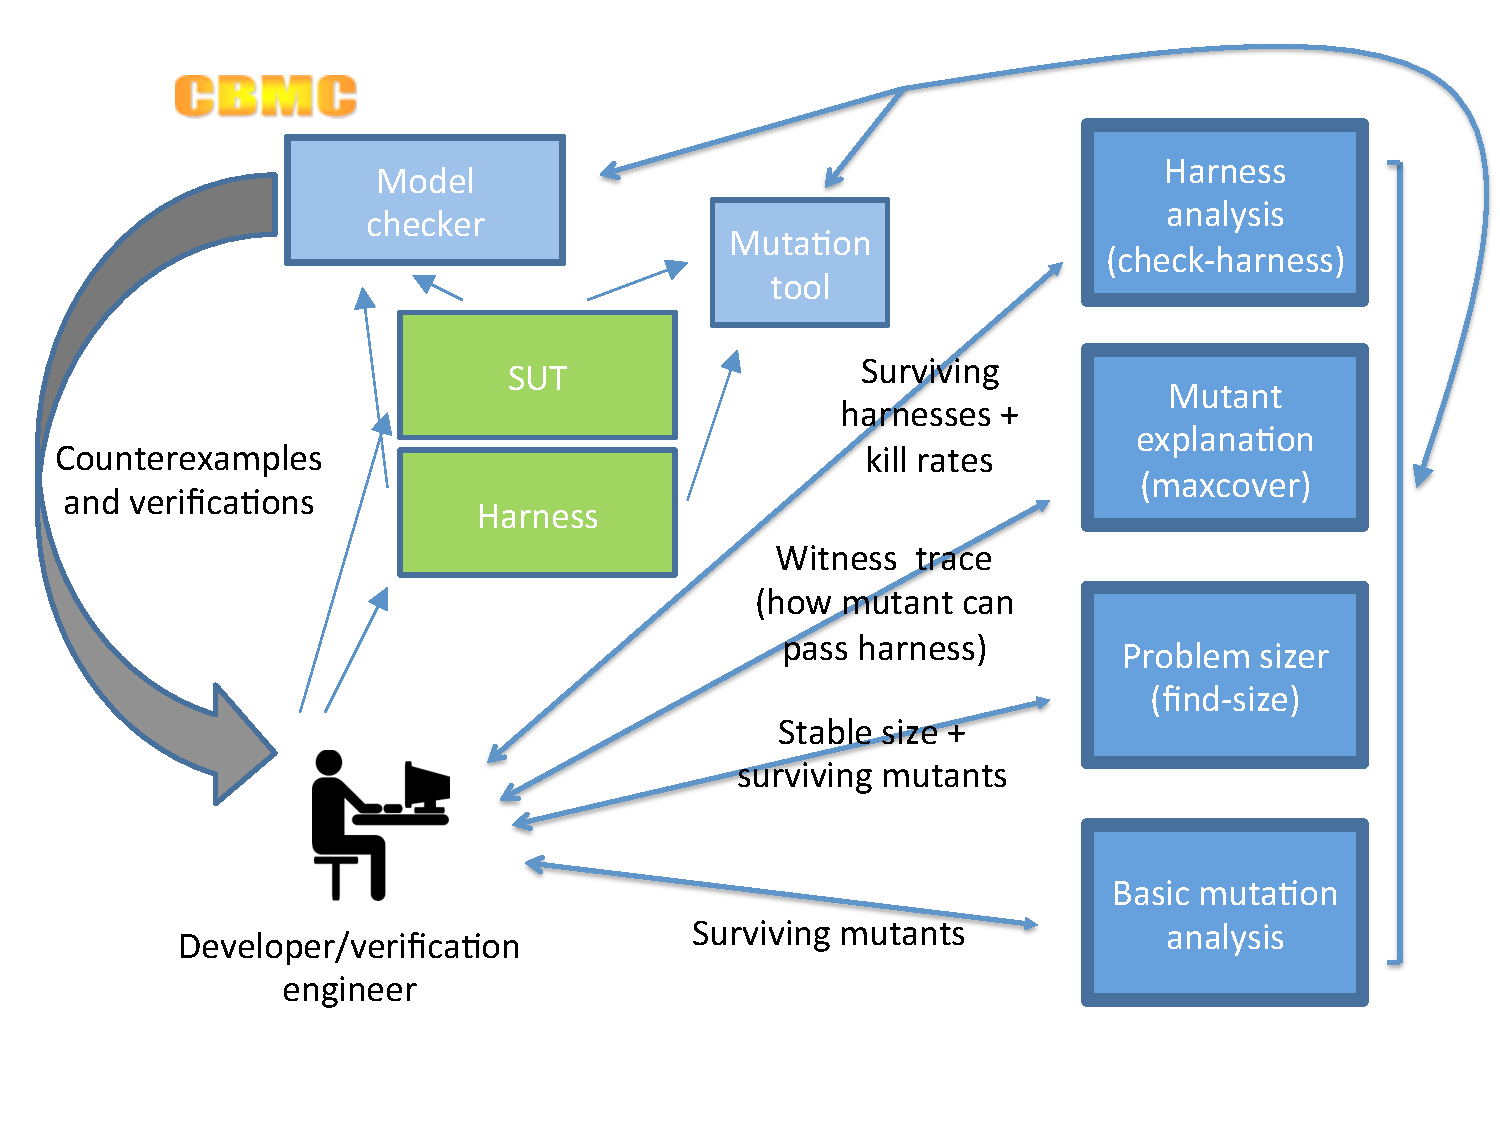
\includegraphics[width=\columnwidth]{TestFlow}
\caption{Basic flow of falsification-driven verification.}
\label{fig:flow}
\end{figure}

\begin{figure}
{\scriptsize 
\begin{code}
(int, survivors) find-size($H$, $M$, $S_0$: int,
                           $O$: int $\rightarrow$ options,
                           $U$: int $\rightarrow$ int) 
\vspace{0.1in}
S = $S_0$-1 
r' = \{\}
changed = False 
while changed:
   TOP:
   S = S + 1 
   changed = False 
   r = r' 
   r' = \{\}
   for $m \in M$:
      if $m \not\in r$:
         r[m] = check($H$,$m$,$U(S)$,$O(S)$) 
         if r[m] == VERIFICATION FAILED:
            //once killed, assume always killed 
            $M$ = $M \\ m$
      if r[m] == VERIFICATION SUCCESSFUL:
         r'[m] = check($H$,$m$,$U(S+1)$,$O(S+1)$) 
         if r'[m] == VERIFICATION FAILED:
            $M$ = $M \\ m$
            changed = True 
            goto TOP 
// No result changed, so S is mutant-stable 
return (S-1, $M$) 
\end{code}
}
\caption{Algorithm 1: Finding size/unwinding bound and surviving mutants.}
\label{alg:unwind}
\end{figure}

\begin{figure}
{\scriptsize 
\begin{code}
harness covering($H$, $TARGET$) 
\vspace{0.1in}
$H'$ = $H$

for stmt $\in H'$:
   if stmt == assert(P):
      stmt = assume(P);

cover = [
  assume(total\_coverage >= $TARGET$); 
  assert(!mutant\_covered);
]

insert cover at end of $H'$.main() 

return $H'$
\end{code}
}
\caption{Algorithm 2: Convert harness into maximal coverage search.}
\label{alg:invert}
\end{figure}

\begin{figure}
{\scriptsize 
\begin{code}
mutant coverinst($m$) 
\vspace{0.1in}
n = 0
$m'$ = $m$
for if\_stmt c in $m'$:
   if c has no else:
      add [else \{\}] to c
for basic\_block b in $m'$:
   b = [if !covered[n] \{
           covered[n] = 1;
           total\_covered += 1;
        \}
        b]
   n = n + 1
for stmt s in $m'$:
   if MUTANT(s):
      s = [\{mutant\_covered = 1;
            s\}]
$m'$ = [int total\_covered = 0;
      int mutant\_covered = 0;
      int covered[n];
      $m'$]

return $m'$
\end{code}
}
\caption{Algorithm 3: Instrument mutant for coverage.}
\label{alg:covermut}
\end{figure}

\begin{figure}
{\scriptsize 
\begin{code}
trace maxcover($m$, $H$, $S$, $O$, $U$) 
\vspace{0.1in}

$m'$ = coverinst($m$)

T = 0
trace = $\emptyset$
failed = False
while (not failed)
   $H'$ = covering($H$, T)
   r = scheck($H$,$m'$,$U(S)$,$O(S)$)
   if r == VERIFICATION SUCCESSFUL:
     // Can't achieve this level of coverage
     failed = True
   else if r == VERIFICATION FAILED:
     trace = r.trace
     // Instead of incrementing by 1, see
     // what actual coverage was and
     // increase by one from that baseline.
     T = trace.read(total\_covered) + 1
return trace
\end{code}
}
\caption{Algorithm 4: Find a maximally covering execution trace that
  covers a mutant.}
\label{alg:maxcover}
\end{figure}

\begin{figure}
{\scriptsize 
\begin{code}
report check-harness($SUT$, $M$, $H$, $M(H)$, $S$, $O$, $U$) 
\vspace{0.1in}

K$_H$ = killed($M$, $H$, $S$) 

Hkills = $\emptyset$
Hequal = $\emptyset$
Hbetter = $\emptyset$

for H$_i$ in $M(H)$:
   original = check($H_i$, $SUT$, $U(S)$, $O(S)$)
   // ``kills'' the SUT -- an invalid harness
   if original == VERIFICATION FAILED: 
      Hkills += H$_i$
   else: // check if this kills fewer mutants
      K$_{H_i}$ = killed($M$, $H$, $S$)
      if |K$_{H_i}$| > |K$_H$|:
         Hbetter += H$_i$
      if |K$_{H_i}$| == |K$_H$|:
         Hequal += H$_i$
      else:
         Hkills += H$_i$
return (Hkills, Hequal, Hbetter)
\end{code}
}
\caption{Algorithm 5: Analyze a harness.}
\label{alg:checkharness}
\end{figure}

\begin{comment}
\begin{figure}
{\scriptsize
\begin{code}
int main () \{
  int a[SIZE], b[SIZE], c[SIZE*2];
  int i, v, i1, i2, csize;
  int asize = nondet\_int();
  int bsize = nondet\_int();
  \_\_CPROVER\_assume ((asize >= 0) \&\& (bsize >=0));
  \_\_CPROVER\_assume ((asize <= SIZE) \&\& (bsize <= SIZE));
  for (i = 0; i < asize; i++) \{
    a[i] = nondet\_int();
    \_\_CPROVER\_assume((i == 0) || (a[i] >= a[i-1]));
  \}
  for (i = 0; i < bsize; i++) \{
    b[i] = nondet\_int();
    \_\_CPROVER\_assume((i == 0) || (b[i] >= b[i-1]));
  \}
  csize = merge\_sorted\_nodups(a, asize, b, bsize, c);
  assert (csize <= (asize + bsize));
  i1 = nondet\_int();
  i2 = nondet\_int();
  \_\_CPROVER\_assume((i1 >= 0) \&\& (i2 >= 0));
  \_\_CPROVER\_assume((i1 < csize) \& \& (i2 < csize));
  \_\_CPROVER\_assume(i1 != i2);
  assert(c[i1] != c[i2]);
  v = nondet\_int();
  \_\_CPROVER\_assume ((v >= 0) \&\& (v < asize));
  v = a[v];
  int found = 0;
  for (i = 0; i < csize; i++) \{
    if (c[i] == v)
      found = 1;
  \}
  assert (found == 1);
  v = nondet\_int();
  \_\_CPROVER\_assume ((v >= 0) \&\& (v < bsize));
  v = b[v];
  int found = 0;
  for (i = 0; i < csize; i++) \{
    if (c[i] == v)
      found = 1;
  \}
  assert (found == 1);
\}
\end{code}
}
\caption{Harness for merge\_sorted\_nodups}
\label{fig:mergeharness}
\end{figure}

\begin{figure}
{\scriptsize
\begin{code}
int merge\_sorted\_nodups(int a[], int asize, 
                        int b[], int bsize, int c[]) \{
  int apos = 0, bpos = 0, cpos = -1, csize = 0;
  while ((apos < asize) || (bpos < bsize)) \{
    if ((apos < asize) \&\& 
        ((bpos >= bsize) || (a[apos] < b[bpos]))) \{
      if ((cpos == -1) || (c[cpos] != a[apos])) \{
	c[++cpos] = a[apos];
	csize++;
      \}
      apos++;
    \} else \{
      if ((cpos == -1) || (c[cpos] != b[bpos])) \{
	c[++cpos] = b[bpos];
	csize++;
      \}
      bpos++;      
    \}
  \}
  return csize;
\}
\end{code}
}
\caption{Code to merge two sorted arrays into one sorted array with no
  duplicate elements}
\label{fig:sortnodup}
\end{figure}
\end{comment}

\begin{comment}
Given a mutant of program $P$, $M_i$, the 

Even a killed mutant (e.g., a mutant the harness detects) can shed
critical light on harness vulnerabilities.  For example, the code in
Figure \ref{fig:mergeharness} is a portion of a harness to verify
code that merges two sorted arrays, removing all duplicates (the
source arrays may contain duplicates or shared items, the output array
is guaranteed to be sorted and have all-unique values).  This harness
detects all non-equivalent mutants of the source code.  However, as is
well known, many software faults \cite{justmutants} are not
represented by a mutant.  Because we are model checking, we want our
harness to actually rule out \emph{all} bad runs of the program under
test.  Even a killed mutant's passing executions may show such a
problem.  Here we see that when the output array's size is 1, the way
we have written the duplicate check in fact \emph{assume}s away
\emph{all executions}!  We check no properties of size 1 output
arrays, and a fault that only appears with size = 1 will never be
detected.  No mutant produces such behavior, but noting an incorrect
but passing trace of this run lets us see the problem.
\end{comment}

\section{Case Studies and Experimental Results}

\subsection{Algorithm Implementations}

Our initial experiments involved relatively small verification
problems, based on implementations taken from the web or student code for popular
algorithms and data structures.  Here we highlight the most
interesting of these; we also successfully applied the method to
bubble sort, a duplicate-removing array merge function, an AVL
tree, and a student's harness for verifying a version of Dijkstra's
shortest path algorithm that enables path reconstruction \cite{dijkstrasp}.  In the case of the AVL tree, the harness we were working with
was unable to reach a mutant-stable unwinding without exhausting
memory on the verification of the main program (for AVL trees of up to
size 5).  We are investigating a more efficient harness encoding,
based on the inability to reach mutant-stability.  For the Dijkstra
harness, the low mutant kill rate of only 58\% showed that while the
harness checks incorrect returned paths, it cannot detect when return
values indicate there is no path but one exists.  Improving the
harness is a substantial exercise, but can be guided by the survival witnesses.

\subsubsection{Binary Search}

The ideas in this paper grew out of a side project of the first
author: to write a follow-up to Jon Bentley's article on verifying
binary search \cite{Bentley} in the context of modern software
verification tools (and Joshua Bloch's discovery of a bug in the
assumptions behind Bentley's proof \cite{Bloch}).  The modeling
required is moderately complex (to scale well, an abstract ``sorted
array'' that represents all sorted arrays but only introduces
variables equal to the number of probes made by the search is
essential).  In this case, we did not produce an initial, weaker
version of the harness, but checked the existing harness using
mutants, and determined that all 3 surviving mutants are equivalent to
a true binary search.

Checking harness mutants (which took 37 minutes, including computing
the kills for the original harness) produced results confirming the belief this is a
good harness.  Of the 31 compiling harness mutants, 19 failed to verify
the correct binary search, and 7 had worse kill rates than the
original harness.  The remaining 5 harnesses, all with equal kill
rates of 86.7\%, all modify an assumption to allow the harness to also
check size 0 arrays.  This doesn't kill any additional mutants, but is
harmless as expected.  Of the harness mutants with worse kill rates,
three are mutants of the assumptions on the nondeterministic value used to
make sure that if binary search returns -1, no index in the array
actually contains the searched-for item.  Two of these mutants are
off-by-one-errors that exclude item 0 from the check, an easy-to-make
mistake.  Both of these fail to kill \emph{exactly} one mutant killed by the
correct harness: the mutant that sets the lower bound
initially to 1 instead of 0.  Traces of passing runs for these mutants show the
problem clearly (the sought item at index 0).

\subsubsection{Doubly-linked-list Insertion Sort}

Another example, making use of recursive data structures and pointer
validity checks, is code for inserting an item (in
sorted order) into a doubly-linked list \cite{DLLInsert}.  Our initial
harness omitted a check for correctness of {\tt prev} pointers.  This
problem didn't directly prevent mutants from being detected, but
pushed the stable size larger, as with the quicksort example above.
Looking at a trace of a size 3 run that fails to kill a clearly
problematic mutant easily reveals the problem (the results are correct
up to {\tt prev} pointers).  This example also showed another use of
mutants, in that some seemingly problematic surviving mutants actually
just showed a pointless redundancy in the implementation, enabling the
removal of an entire conditional branch.  A harness check (requiring
30 minutes, including computing the mutant kills for the original
harness) showed that of the 105 compiling harness mutants, 92 fail to
verify the original code.  Another 2 have a worse kill rate than the
original (which kills 81\% of mutants, a low rate due to the code
redundancy), and 11 survive.  The large number of survivors is due to
a redundancy of the final harness, which checks sortedness and the
permutation property for both a forward {\tt next} traversal of the
list and a {\tt prev} traversal.  Omitting any \emph{one} of these
(e.g. {\tt prev} sortedness or {\tt next} permutation) the harness can
still detect all mutants.  Removing two, however, fails to kill
mutants.  The two harness mutants with worse kill rates have extremely poor
kill rates ($<50$\% and $<25$\%).
%\subsubsection{AVL Tree}


%\subsubsection{Merge With Duplicate Removal}

\subsection{SpiderMonkey Boyer-Moore-Horspool Implementation}

\begin{figure}
{\scriptsize
\begin{code}
jsint
js\_BoyerMooreHorspool(const jschar *text, jsint textlen,
                      const jschar *pat, jsint patlen,
                      jsint start)
\{
  jsint i, j, k, m;
  uint8 skip[BMH\_CHARSET\_SIZE];
  jschar c;

  JS\_ASSERT(0 < patlen && patlen <= BMH\_PATLEN\_MAX);
  for (i = 0; i < BMH\_CHARSET\_SIZE; i++)
    skip[i] = (uint8)patlen;
  m = patlen - 1;
  for (i = 0; i < m; i++) \{
    c = pat[i];
    if (c >= BMH\_CHARSET\_SIZE)
      return BMH\_BAD\_PATTERN;
    skip[c] = (uint8)(m - i);
  \}
  for (k = start + m;
       k < textlen;
       k += ((c = text[k]) >= BMH\_CHARSET\_SIZE) ? 
             patlen : skip[c]) \{
    for (i = k, j = m; ; i--, j--) \{
      if (j < 0)
	return i + 1;
      if (text[i] != pat[j])
	break;
    \}
  \}
  return -1;
\}
\end{code}
}
\caption{SpiderMonkey 1.6 Boyer-Moore-Horspool code.}
\label{fig:bmh}
\end{figure}

\begin{figure}
{\scriptsize
\begin{code}
\#include "bmh.h"
int main() \{
  int i;
  unsigned int v;

  char itext[TSIZE];
  char ipat[PSIZE];

  unsigned int itext\_s = nondet\_uint();
  \_\_CPROVER\_assume(itext\_s < TSIZE);
  unsigned int ipat\_s = nondet\_uint();
  \_\_CPROVER\_assume(ipat\_s < PSIZE);

  printf ("LOG: size text=\%u, pat=\%u\\n", itext\_s, ipat\_s);

  for (i = 0; i < itext\_s; i++) \{
    v = nondet\_unit();
    \_\_CPROVER\_assume((long)v < (long)BMH\_CHARSET\_SIZE);
    itext[i] = v;
    \_\_CPROVER\_assume(itext[i] < BMH\_CHARSET\_SIZE);
    printf ("LOG: text[\%d] = \%u\\n", i, itext[i]);
  \}

  for (i = 0; i < ipat\_s; i++) \{
    v = nondet\_uint();
    \_\_CPROVER\_assume((long)v < (long)BMH\_CHARSET\_SIZE);
    ipat[i] = v;
    \_\_CPROVER\_assume(ipat[i] < BMH\_CHARSET\_SIZE);
    printf ("LOG: pat[\%d] = \%u\\n", i, ipat[i]);
  \}

  jsint r = js\_BoyerMooreHorspool(itext, itext\_s, 
                ipat, ipat\_s, 0);

  printf ("LOG: return = \%d\\n", r);
  
  int pos, ppos, found;

  v = nondet\_uint();
  printf ("LOG: looking at \%u\\n", v);
  \_\_CPROVER\_assume(v >= 0);
  
  if (r == -1) \{
    \_\_CPROVER\_assume(v < itext\_s);
    pos = v; ppos = 0; found = 1;
    while (ppos < ipat\_s) \{
      printf ("LOG: itext[\%d] = \%u, ipat[\%d] = \%u\\n",
                 pos, itext[pos], ppos, ipat[ppos]);      
      if ((pos>=itext\_s)||(itext[pos]!=ipat[ppos])) \{
	found = 0; break;
      \}
      pos++; ppos++;
    \}
    assert (!found);
  \} else \{
    pos = r; ppos = 0;
    while (ppos < ipat\_s) \{
      assert (itext[pos] == ipat[ppos]);
      pos++; ppos++;
    \}
    v = nondet\_uint();
    printf ("LOG: looking at \%u\\n", v);
    \_\_CPROVER\_assume(v < r);
    pos = v; ppos = 0; found = 1;
    while (ppos < ipat\_s) \{
      printf ("LOG: itext[\%d] = \%u, ipat[\%d] = \%u\\n",
                 pos, itext[pos], ppos, ipat[ppos]);
      if ((pos>=itext\_s)||(itext[pos]!=ipat[ppos])) \{
	found = 0; break;
      \}
      pos++; ppos++;
    \}
    assert (!found);
  \}
\}
\end{code}
}
\caption{Boyer-Moore-Horspool harness.}
\label{fig:bmhharn}
\end{figure}

Figures \ref{fig:bmh} and \ref{fig:bmhharn} show, respectively, the
source code and an initial harness for verification of the
Boyer-Moore-Horspool substring finding algorithm \cite{BMH,CFV13} in
version 1.6 of Mozilla's SpiderMonkey JavaScript engine.  Verifying
this code presents one immediate issue that is not unusual in
verification: how to handle an {\tt assert} in the code being
verified.  An {\tt assert} at the end of a function or in the main
body is typically an additional part of the specification, and is
often best left unchanged.  An {\tt assert} at the beginning of a
function's body, however, is typically a precondition for the code \cite{CFV13}.  It is natural to consider changing such an assertion into
an {\tt assume} and ignoring any problems produced by calling the code
with non-conforming inputs.  While this can be a useful technique (for
instance when it is hard to write a harness that only produces valid
inputs, but easy to filter out the invalid inputs and only verify
behavior for those) it is also a dangerous technique.  Mutation
analysis of the harness shows that 4 is a mutant-stable size (where
the same size is used for text length, pattern length, and character
set size), with a kill rate of 72.3\%.  On initial examination, the 20
surviving mutants do not seem problematic.  A large number involve the
{\tt JS\_ASSERT} converted to a {\tt \_\_CPROVER\_assume}, showing the
harness cannot tell if the assumption is incorrect, which is not
surprising (the harness only generates good inputs, and some of the
mutants simply discard too many inputs).

At this point, we were satisfied with our harness, and ran a check on
mutants of the harness itself.  To our surprise, three mutants of the
harness had a \emph{better} kill rate than the ``correct'' harness,
killing 73.5\% of mutants.  Investigating these ``better'' harnesses
showed mutants that broke processing of some return values in such a
way that, while these harnesses failed to detect certain major bugs
in the code, they were able to detect some {\tt JS\_ASSERT} assumption mutants.  Guided
by this, we produced a revised harness that raised the kill rate to
79.52\%.  However, on examining the surviving mutants, we realized
that our verification was still unsatisfactory as a good regression for the
Boyer-Moore-Horspool code:  in particular, if the assertion were ever
modified to allow bad inputs to pass through, or otherwise incorrectly
changed, we would miss some mutants.  We then changed the {\tt
  JS\_ASSERT} into code that returned a special value to signal
assertion failure, and modified the harness once more,
allowing some incorrect values to pass through and checking that
``assertion failure'' happened if, and only if, the inputs were invalid.
This harness killed 89.2\% of mutants, and the six surviving mutants
were easily understood to be equivalent to the BMH code under all
valid inputs (in one case we weren't certain about, we had CBMC verify
that for all non-assertion violating inputs, this was true up to a
large bound).  The new harness, informed by the harness mutations, in
fact had a better mutant kill rate for size 3 (80.7\%) than our first harness
had at the mutant-stable point.  This examples serves as our best
evidence of the value of harness mutation.

\subsection{Linux Kernel RCU Verification Challenges}

%\subsubsection{Introduction to RCU}


RCU is a synchronization mechanism sometimes used as a replacement
for reader-writer locking for linked structures, allowing extremely
lightweight readers \cite{McKenney:2013:SDS:2483852.2483867}.
In the limiting case, achieved in server-class builds of the
Linux kernel, overhead for entering and exiting an \emph{RCU read-side
critical section} (using {\tt rcu\_read\_lock()} and {\tt rcu\_read\_unlock()},
respectively) is exactly zero \cite{McKenney98}, making RCU an
excellent choice for read-mostly workloads \cite{McKenney:2013:SDS:2483852.2483867,DinakarGuniguntala2008IBMSysJ,PaulMcKenney2013AMPenergyHOTPAR}.
However, lightweight readers imply that updaters cannot exclude readers,
so must take care to avoid disrupting readers.
Updaters typically maintain multiple versions of the portion of the
data structure being updated, removing old versions only when
readers are no longer accessing them.
To this end, RCU provides {\tt synchronize\_rcu()}, which waits for a
\emph{grace period}: when all pre-existing RCU readers complete.
RCU updaters typically remove a data element (rendering it
inaccessible to new readers), invoke {\tt synchronize\_rcu()},
and then reclaim a removed element.
\begin{comment}Production-quality implementations of {\tt synchronize\_rcu()} use batching
techniques to achieve extremely scalability, so that a single underlying
grace period can satisfy more than 1,000 concurrent updates in the
Linux kernel~\cite{Sarma04c}.\end{comment}
The Linux kernel contains more than 10,000 uses of the RCU
API \cite{PaulEMcKenneyRCUusagePage}, and a userspace RCU
library \cite{MathieuDesnoyers2009URCU,MathieuDesnoyers2012URCU}
is seeing significant use.  Validation and verification of RCU is a
major concern for each implementation, and a topic of considerable
interest in the PL/verification community now \cite{PLDI15RCU}.

\begin{comment}
\emph{Should we cite this? 
\url{http://conf.researchr.org/event/pldi2015/pldi2015-papers-verifying-read-copy-update-in-a-logic-for-weak-memory}}
\end{comment}


\begin{comment}{The {\tt rcutorture} stress-test suite qualifies, but it would be
good to evaluate its effectiveness on the one hand
(via permutation analysis)
and to include formal verification on the other.
However, regression-test use of formal verification required that
the following properties:
(1)~Direct use of source code,
(2)~Automatic discarding of irrelevant source statements,
(3)~Reasonable memory and CPU overhead,
(4)~Automatic mapping of error reports to source lines, and
(5)~Modest additional input beyond the source code.
Failing to provide any of these requirements provides unacceptable
vulnerability to human error.
This raise the question of whether readily available formal-verification
tools meet these requirements.}
\end{comment}

\begin{figure}[tb]
{ \scriptsize
\begin{verbatim}
 1 static int rcu_read_nesting_global;
 2 
 3 static void rcu_read_lock(void)
 4 {
 5   (void)__sync_fetch_and_add(&rcu_read_nesting_global, 2);
 6 }
 7 
 8 static void rcu_read_unlock(void)
 9 {
10   (void)__sync_fetch_and_add(&rcu_read_nesting_global, -2);
11 }
12 
13 static void synchronize_rcu(void)
14 {
15   for (;;) {
16     if (__sync_fetch_and_xor(&rcu_read_nesting_global, 1) < 2)
17       return;
18     SET_NOASSERT();
19     return;
20   }
21 }
\end{verbatim}
}
\caption{Approximate model of RCU}
\label{fig:Approximate Model of RCU}
\end{figure}

Because both RCU and the Linux kernel are moving targets, any validation
and verification must be both automated and repeatable, for inclusion
in a regression-test suite.  At present the {\tt rcutorture}
stress-test provides some assurance in the form of automated testing,
but ideally would be complemented by some formal verification of the
implementation(s) in the kernel.  An important question is whether
available formal verification tools can provide effective additional
regression checking for RCU.
We use a pair of RCU-related benchmarks \cite{PaulBlog1,PaulBlog2} to
provide the beginnings of an answer to this question.  The first
benchmark applies formal verification to the simplest of the Linux
kernel's RCU implementations, Tiny RCU
\cite{PaulEMcKenney2009BloatwatchRCU}, which targets single-CPU
systems.  This model includes Tiny RCU's handling of idle CPUs as well
as its (trivial) grace-period detection scheme.  The second benchmark
creates the trivial model approximating an RCU implementation for
multiprocessor systems shown in Figure \ref{fig:Approximate Model of
  RCU}.  In this model, the number of RCU read-side critical sections
currently in flight is tracked by the global
{\tt rcu\_read\_nesting\_global}, which is atomically incremented by
{\tt rcu\_read\_lock()} and atomically decremented by
{\tt rcu\_read\_unlock()}.  This allows {\tt synchronize\_rcu()} to
atomically XOR {\tt rcu\_read\_nesting\_global}'s bottom bit to detect
whether the current execution has waited for all pre-existing readers
(over-approximated by checking the absence of all readers), with
{\tt SET\_NOASSERT()} being invoked to suppress all future assertions.
Although this model has a number of shortcomings, perhaps most
prominently excessive read-side ordering, it is capable of detecting
common RCU-usage bugs, including failure to wait for an RCU grace
period and failure to enclose read-side references in an RCU read-side
critical section.  Can falsification aid in these two complex,
in-progress, verification efforts?

Our efforts are ongoing, due to the complexity of the targeted code
(even with support from the primary developer, a co-author of this
paper).  At this time the
investigation of mutants has already provided valuable information
about these verifications benchmarks.  First, there are two versions
of the Tiny RCU verification.  The earliest, very preliminary version,
kills only 10 of 169 Tiny RCU mutants.  Adding code to the harness to
account for interrupts in the dyntick-idle handling kills an
additional 12 mutants, confirming that the modification increases the
strength of the harness.  More importantly, the modeling of
concurrency in the harness has two versions, one using CBMC support
for pthread mutex locks, the other using disabling of assertions to
ignore executions that violate locking semantics.  The native mutex
version allows much faster verification, and catches the original,
hand-constructed checks to ensure the harness can detect faults in
Tiny RCU.  However, the native mutex version fails to kill \emph{any}
mutants, a fact we are currently investigating:  without mutants, we
would not have been aware of this possibly critical problem, which may
be a CBMC bug (in the course of this paper's work, we have uncovered
several CBMC bugs) or a harness flaw.  In support of the
verification, we also generated passing maximal-coverage executions for all
mutants of the Tiny RCU code.  For 97 of the mutants, there is no
passing execution; in many cases, these are not killed: the mutant
modifies the concurrency semantics so CBMC has no valid executions to
analyze (potentially invalid in some cases, which must be
investigated).  For 79 mutants the maximal-coverage passing runs are
currently being examined, to determine the best next steps in
improving the Tiny RCU harness.
For the second benchmark, we have computed mutant kills and find that
the kill rates range between 40\% and 46\%.  While these benchmarks
are far from complete, and over-simplify the modeling process, they
are already able to catch a substantial number of potential RCU usage
errors.  Again, we have produced passing runs for the surviving
mutants to use in enhancing the process.  The good news is that while
the RCU verification is much more substantial than the above case
studies, the time to analyze mutants is not prohibitive.  No single
model checking run for the Tiny RCU benchmark takes more than 40
seconds, and \emph{total runtime} for all mutants in the usage
benchmarks ranges from just over 12 seconds for a basic litmus test to
less than 5 minutes for the most complex of the benchmarks.


\begin{comment}
Nevertheless, it is important to note that these two benchmarks are not
examples of useful verifications, but rather the simplest examples of
a class that might some day expand to include useful verifications.

(And of course, CBMC proved capable of handling simple variable-pair
litmus tests, as well as single-threaded examples involving linked lists,
but proved incapable of handling multi-threaded tests involving linked
lists.
The maintainers of CBMC are working to improve its handling of pointers.)
\end{comment}

\subsection{Experiments: Plausible Verification by Failure to Falsify}
\label{sec:sattimes}

\begin{figure}
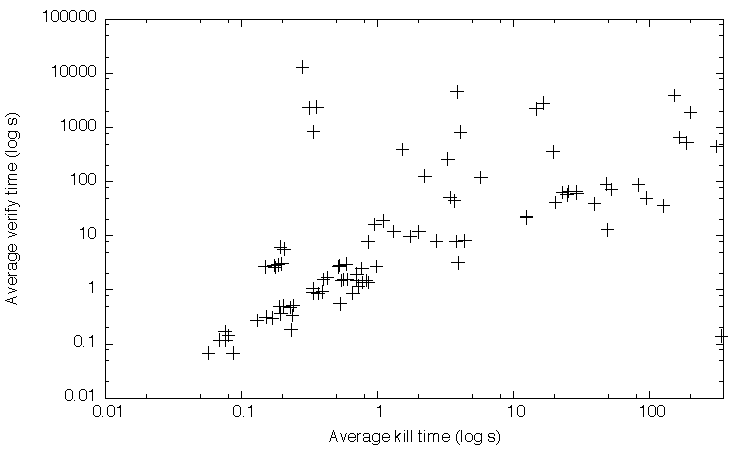
\includegraphics[width=\columnwidth]{sattimes}
\caption{Average times for killed mutants (SAT) vs. surviving mutants 
  (UNSAT) for all experiments.}
\label{fig:sattimes}
\end{figure}

A key problem in model checking is the state explosion problem, or,
more simply (and more accurately, in that number of states is not
always the determining factor in symbolic methods) the problem of
scalability.  As discussed above, even proving binary search correct
over the full domain of integer inputs is not possible within a
reasonable time frame.  Even when verification is impossible at the
desired problem size falsification can provide limited
confidence in the correctness of a program.  In particular, we observe
from all of our experiments that the average time, for any program and
harness pair, to verify the original code and all surviving mutants is
\emph{much higher} than the average time to produce a counterexample
for killed mutants.  Showing that a constraint is satisfiable is,
usually, easier than proving it is unsatisfiable.  This is not limited
to SAT solvers; we used SAT rather than SMT in our experiments because
we generally found Z3 to be slower than CBMC's built in version of
MiniSAT\cite{minisat} in almost all cases, but Z3 also
aims to be fast at producing satisfying assignments, not proving UNSAT
\cite{z3}, and our few runs with Z3 showed the same pattern.

Figure \ref{fig:sattimes} shows (with log scales on both axes) the
average running times for all experiments (including faulty versions
of the harness, incorrect runtime parameters, harness mutation checks,
etc.) performed in the course of this work.  The general trend is
clear: time to verify is usually worse than time to kill, and the
worst average time to kill (about 350 seconds) is much better than
many average verification times.  One use of this relationship is
that, in cases where all (non-equivalent) mutants of the SUT are
killed, but the SUT verification fails to complete, the SUT might be
considered \emph{provisionally} verified. In particular, the larger
the ratio between the timeout for failed verification and the longest
kill time for any mutant, the ``more likely'' to be correct we can
consider the SUT (the same holds with respect to memory use
limits). This belief can be further justified by modifying the harness
to force mutant kills to use large problem sizes, violating the usual
inclusiveness rule (that way, if the new size allows a counterexample
not previously existing, the mutant killing problem for mutants
killable at smaller sizes better approximates the counterexample
construction problem for the actual fault).

Additionally, the times shown here (with mean mutant kill time of 16.4
seconds and median mutant kill time of 0.54 seconds) show the general
feasibility of the falsification-driven approach.  Most of the time,
killing mutants is cost-effective.  The outliers come from a few
difficult problems, arising from buggy harnesses (or harness mutants
that resemble buggy harnesses).  The much worse cost for surviving
mutants is due to a few expensive stubborn mutants: the median
verification success time is only 1.5 seconds.

\section{Discussion}

\subsection{Falsification vs. Verification}

The core idea of this paper is that, while successful verification is
the \emph{result} that a developer seeks when verifying a program, it
is most meaningful in a context provided by many failed verifications.
The useful model checking harness (e.g., specification) essentially,
is one that \emph{prohibits} certain execution sequences.  This is not
controversial; a good property is defined by its rejection of bad
behavior.  However, in most verification efforts, there is a focus on
arriving at a successful verification, which sheds very little light
on exactly \emph{what} has been verified.  By focusing on mutants throughout the
verification process, our approach shifts the emphasis to one of
``verifying'' the verification itself by repeatedly \emph{falsifying}
claims that various incorrect programs satisfy the property.  This is,
at a conceptual level, akin to Karl Popper's philosophy of science
\cite{Popper}.

For Popper, all scientific knowledge is provisional, and the key to
the scientific approach is a critical effort, based on
\emph{prohibitive} theories.  In brief, Popper proposes that proper
science must be strongly grounded in a search for counterexamples.
Using mutants as a basis for verification is akin to this approach,
with the harness taken to be the ``theory'' of the empirical behavior
of the world.  Mutants, in this view, are counterfactual worlds that
are likely to violate any correct theory of the actual world.  A
``scientific theory'' (that is, a harness) is proven effective by its
ability to be \emph{shown to be false} in these counterfactual worlds.
If we can prove a theory is incorrect for an ``incorrect'' world and
cannot prove it is incorrect for the real world, that gives us greater
confidence (always provisional, since our understanding of the world,
e.g., any complex software system, is almost always limited and prone
to error) that the theory is indeed true of the real world/program.
Of course, generating alternative worlds and showing that, for
example, special relativity is easily falsified in a world where
special relativity does not in fact hold, is not practical in
scientific discovery.  It is, however, quite easy in the artificial
``scientific discovery'' sense of verifying properties of computer programs.

\subsection{The Power of Exhaustive Nondeterminism}

The ability to improve a harness based on surviving mutants (or on
passing runs of killed mutants) essentially relies on the nature of
exhaustive bounded model checking based on constraint solving.  In
non-exhaustive automated testing, the answer to why a mutant is not
killed is, often, neither ``the oracle is not good enough'' nor even
``the test process is inadequate and needs to be modified'' but ``you
didn't get lucky.''  That is, killing all mutants is, in many cases,
not something we can expect of non-exhaustive test suites.  Random
testing \cite{HamletOnly,ICSEDiff} can perform well in general as a
bug-finding method, but its failure to kill any individual mutant is
likely to be a matter of probability, rather than a flaw \emph{per se}
in the testing itself.  In verification, however, there are no
accidents: if a harness verifies an incorrect program, either the
assumptions, the specification, or the problem size are \emph{necessarily} in
need of correction.  However, the approach we propose is most suited
to the analysis space in which CBMC is situated: on the one hand,
within a known bound, its results are exhaustive; on the other hand,
the method behaves much like a dynamic analysis, in that there are no
false positives.

\section{Related Work}

The idea that a ``successful verification'' in model checking (or even
theorem proving) often simply indicates an inadequate property is
long-standing \cite{PracticalCov,Hoskote}. Use of mutants
\cite{MutSpec,MutCov} to provide a coverage measure dates back both to
these early explorations and relatively recent work \cite{MutInterp}.
However, in these efforts the mutation was usually applied to hardware
models, and (critically) the surviving mutants were used to identify
``uncovered'' portions of a model, rather than presented to a
developer for examination and understanding directly.  To our
knowledge, no previous work presented passing executions of a source
code mutant as a guide to understanding specification weakness.  Our
modification of the harness is a source-code analogue to attempts to
modify logical formulas, e.g., the effort to (in a narrow,
vacuity-based sense) produce the \emph{strongest passing LTL formula}
of Chockler et al. \cite{BeyondVac}.  We are not the first to note
that model checking, at present, due to the ``many obstacles'' in
proving a system correct, is primarily used for falsification
\cite{AbsFals}.  Previous work on the topic \cite{AbsFals} focused on
abstractions based on under-approximation, to ensure counterexamples
were not spurious. We instead preserve the goal of
verification\footnote{Note that we use a model checking approach that
  already guarantees non-spurious counterexamples, and provides
  bounded rather than full verification.}, but \emph{drive} the verification
process, from the human point of view, by repeated falsification of
incorrect systems.

More distantly related is the general effort to determine the quality
not only of test suites (which is often focused on missing tests
within the ``range'' of testing, not a problem for CBMC) but of test
oracles and entire testing infrastructures.  The problem of ``testing
the tester'' \cite{WODA09} is fundamental to all efforts
to improve software quality.  Recent efforts of most interest have
focused on measuring \emph{checked coverage} \cite{CheckedCov,CheckedJournal,ThereYet}, where
a metric tries to make sure the code under test potentially changes
the value of an assert, using dynamic slicing \cite{DynSlice,Tip}.  This is weaker than requiring the oracle kill
a mutant, our goal, but more manageable for testing, where complete
behavioral coverage is less feasible than in model checking (and where
source code sizes combined with test inadequacy may make hand mutation analysis infeasible).

\begin{comment}
Our idea of examining successful executions to better understand
surviving (and even killed) mutants is a peculiar variation of the
fault localization and error explanation problem in model checking
\cite{GroceDist}, with the twist being that we are ``explaining'' an
artificial fault that 1) typically does not cause a test failure (for
surviving mutants) and 2) has an obviously known location.
\end{comment}

\section{Conclusions and Future Work}

This paper proposes a \emph{falsification-driven} methodology for
formal verification, particularly when verification is performed by
the developers of critical software systems.  These developers are not
experts in formal verification, but in the systems they are verifying.
Verification is, we claim, always provisional, in that the potential
flaws in our assumptions, specification, and understanding of system
behavior tend to leave room for doubt about the correctness of any
verification result.  Verification of code is not self-explanatory,
unlike a counterexample.  We propose to take advantage of the use of
counterexamples and witnesses and center verification around the
\emph{incorrect programs a verification fails to prove incorrect}.  An
obvious source of such programs is mutants; we also suggest that
known-flawed versions of code be included in this set, which all of
our tools support, but the key to the method is the generation of a
large set of potential buggy versions without developer effort.  Given
these versions, a developer can examine mutants that a verification
effort fails to detect, and (with the algorithms and tools presented
in this paper) examine executions showing precisely how a program
mutant can ``make it through'' a verification without being detected,
with assurance that these executions will have high coverage (and thus
likely be non-trivial).  Developers can also check that a verification
harness does not have any mutants that 1) verify the SUT while 2) killing
\emph{more} mutants than the original harness.  This can help detect
very subtle flaws in harnesses, especially those based on bad
reasoning about ``equivalent'' mutants.  We demonstrate, as a
proof-of-concept, that our approach can be useful for simple but
realistic verification efforts, and can contribute to serious systems
verification and modeling efforts for complex code such as the Linux
kernel RCU implementations.  The bigger picture is that our approach
attempts to apply the ideas of Karl Popper's falsification-centered
approach to the philosophy of science to the understanding of software
systems.  In this view, verification is almost always provisional, but we can 
gain considerable confidence in a verification by making serious attempts to prove its inadequacy.

In future work we plan to continue to apply this falsification-driven
approach to the RCU verification, and to other critical
systems-software targets as well.  In the process we expect to
discover new supporting algorithms and methods that use a model
checker's ability to ask ``what if'' questions about program
executions \cite{GroceDist,MakeMost} to improve developer
understanding of verification efforts.  We would also like to
integrate falsification-driven verification support into the CBMC
Eclipse tools, and use speculative model checking calls and
incremental SAT to make mutant analysis available to developers
continuously as part of their development/debugging process.  Finally,
these techniques should also be applicable to verification using, e.g., Java
Pathfinder \cite{JPF2} (at least in symbolic mode; in pure explicit-state
exploration the problems of non-exhaustive exploration may dominate).

Our CBMC patch for {\tt find-success} mode, the various verification harnesses, and our
experimental results are all available at {\tt \url{https://github.com/agroce/cbmcmutate}}.

% use section* for acknowledgment
%\section*{Acknowledgment}


%
%The authors would like to thank...





% trigger a \newpage just before the given reference
% number - used to balance the columns on the last page
% adjust value as needed - may need to be readjusted if
% the document is modified later
%\IEEEtriggeratref{8}
% The "triggered" command can be changed if desired:
%\IEEEtriggercmd{\enlargethispage{-5in}}

% references section

% can use a bibliography generated by BibTeX as a .bbl file
% BibTeX documentation can be easily obtained at:
% http://www.ctan.org/tex-archive/biblio/bibtex/contrib/doc/
% The IEEEtran BibTeX style support page is at:
% http://www.michaelshell.org/tex/ieeetran/bibtex/
%\bibliographystyle{IEEEtran}
% argument is your BibTeX string definitions and bibliography database(s)
%\bibliography{IEEEabrv,../bib/paper}
%
% <OR> manually copy in the resultant .bbl file
% set second argument of \begin to the number of references
% (used to reserve space for the reference number labels box)
\bibliographystyle{IEEEtran}
\bibliography{bibliography}

% that's all folks
\end{document}
